\newpage
\section{\MakeUppercase{SYSTEM ARCHITECTURE AND METHODOLOGY}}
\subsection{System Architecture}
\begin{figure}[H]
    \centering
    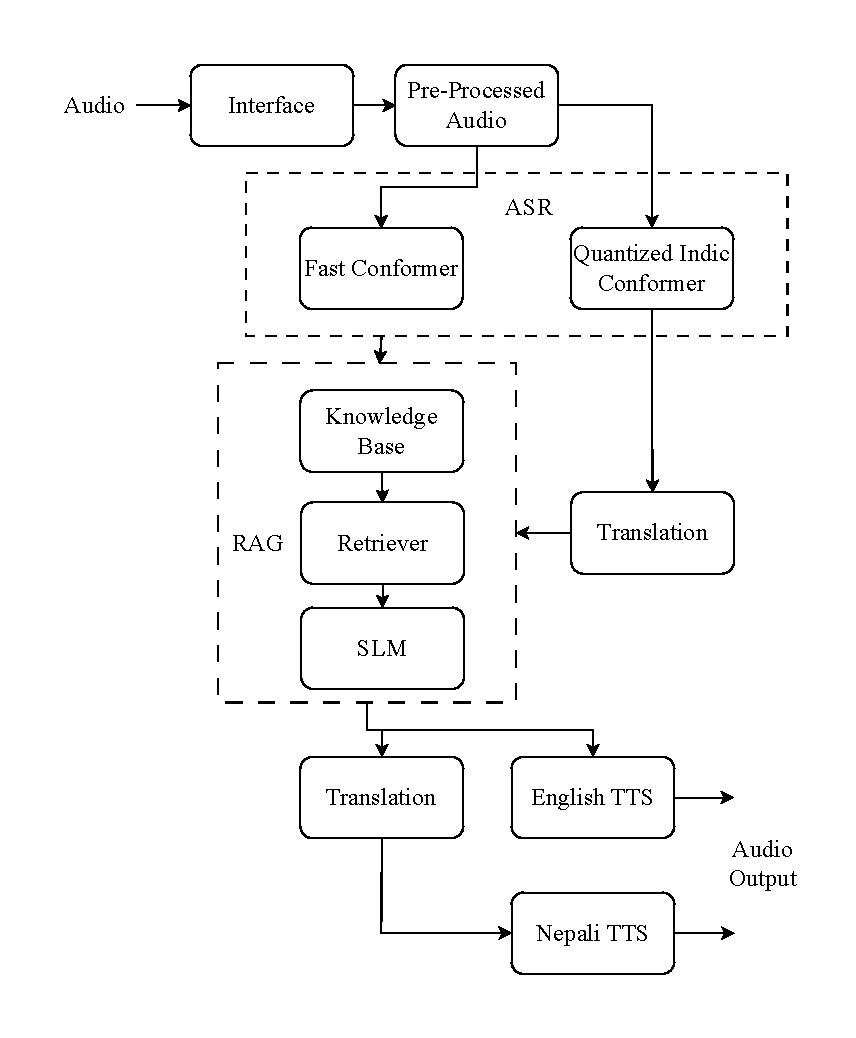
\includegraphics[width=\linewidth]{Images/ASR/Methodology/ASR-SuperMainArchitecture.drawio.pdf}
    \caption{System Architecture}
\end{figure}

The system pipeline starts with the spoken audio of the user that is either in English or Nepali. The Interface module handles the preprocessing of the audio signal after which it is sent to the relevant Automatic Speech Recognition (ASR) pathway depending on which language is being used.In the case of Nepali audio input, the signal is run through the Quantized Indic Conformer model that caters to Indic language meaning that the speech is converted into textual transcription. This transcription is further sent to a Translation module so that it can be translated to English before being sent to the Small Language Model (SLM).With English audio input, the signal is handled in a quicker pathway by the Fast Conformer model that directly transcribes the speech into text. This is an English transcription that is directly forwarded to the SLM without need of translation.The SLM also acts on a Retrieval-Augmented Generation (RAG) basis. It has a Knowledge Base which has the news articles and information of the last two years. When a transcribed text is received by the SLM, the Retriever component is used in a search of this Knowledge Base to retrieve information that is relevant and up-to-date concerning the query made by the user. This memory context is then subjected to the language interpretation abilities of the SLM to create correct responses of context-aware nature based on the latest news and events. The output of the SLM, which is refined on a specialized dataset and optimized to perform local inference, is the combination of the query input and the knowledge retrieved to produce a coherent reply in English.At the end, two output paths are available to the English text response: one of them is to send the English text response straight to the English TTS module and to receive the audio in English and another is to translate the SLM output to nepali and send it to the Nepali TTS module and to get the audio in Nepali. This two-way mechanism offers the system the ability to support bilingual input and offer versatile multilingual output as per the needs of the user.


\subsection{Automatic Speech Recognition}
\subsubsection{Architecture of ASR}
\begin{figure}[H]
    \centering
    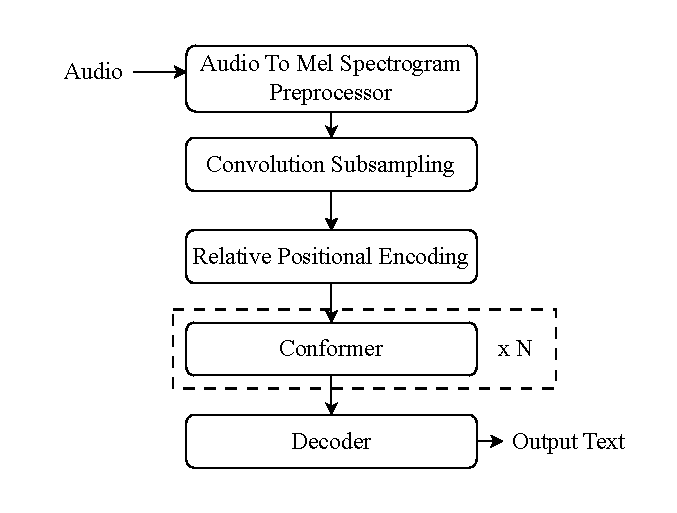
\includegraphics[width=\linewidth]{Images/ASR/Methodology/ASR-Main Architecture.drawio.pdf}
    \caption{Architecture of ASR}
\end{figure}
The ASR subsystem uses two different Conformer-based models to process english and nepali speech input. The FastConformer architecture based on EncDecCTCModelBPE is used to process English speech and the IndicConformer architecture based on EncDecHybridRNNTCTCBPEModel is used to process Nepali speech. Both models are also trained on NeMo benchmarks and have the same overall design, a convolutional front-end, a series of Conformer encoder layers, and a CTC decoding head, but have different model dimensionality, vocabulary size, and encoder layers, since they are trained on different scale data and linguistic complexity data.

\begin{table}[H]
\caption{Model Configuration Comparison: FastConformer (English) vs IndicConformer (Nepali)}
\label{tab:conformer_comparison}
\centering
\small
\begin{tabularx}{\textwidth}{|l|X|X|}
\hline
\textbf{Parameter} & \textbf{FastConformer (English)} & \textbf{IndicConformer (Nepali)} \\
\hline
Model class & \texttt{EncDecCTCModelBPE} & \shortstack[l]{\texttt{EncDecHybrid}\\\texttt{RNNTCTCBPEModel}} \\
Language & English & Nepali (Indic) \\
Encoder hidden dim & 176 & 512 \\
Encoder layers & 16 & 17 \\
FFN expansion ratio & $4\times$ (176 $\to$ 704) & $4\times$ (512 $\to$ 2048) \\
Conv kernel size (depthwise) & 31 & 31 \\
Attention dim & 176 & 512 \\
Vocabulary size & 1025 (BPE) & 5633 (BPE) \\
CTC projection & \texttt{Conv1d(176, 1025)} & \texttt{Conv1d(512, 5633)} \\
Decoding path used & CTC & CTC only \\
\hline
\end{tabularx}
\end{table}

\subsubsection{Feature Extraction}
Both models have the same front end preprocessing pipeline that is an AudioToMelSpectrogramPreprocessor using a FilterbankFeatures featurizer. The raw audio waveforms are converted into mel-frequency filterbank features and these features are then sent to the encoder. Both models use the same technique of the preprocessing pipeline since both are trained on 16 kHz speech data.

\textbf{Sampling Rate}\\
Audio input is resampled to a standard rate of 16,000 Hz (16 kHz) before the extraction of features. This provides consistency in training as well as inference. The frequency range of human speech has most of the perceptually important information in the range of frequencies up to 8 kHz. The Nyquist theorem states that at least 2 x 8,000 = 16,000 samples per second must be used to reproduce frequencies up to 8 kHz with perfect accuracy. 

\textbf{Windowing}
\begin{itemize}
    \item Window Size (25ms)\\
    This defines the time of every frame of time used to calculate spectral features. A 25 ms window provides enough temporal information for speech without at the same time being too local (i.e. less than 25 ms).
    \item Stride \\
    The hop length of 10 ms allows for overlapping frames, which ensures smooth transitions between consecutive feature vectors, capturing fine temporal details.
\end{itemize}

\textbf{Mel-Frequency Features (80 Bin)}
\begin{itemize}
    \item Extracting 80 mel-frequency features allows for a small size yet expressive representation of the audio signal focusing on perceptually relevant frequencies for human speech.
    \item The number of bins balances between resolution and model complexity.
\end{itemize}

\textbf{Logarithmic Scaling}
\begin{itemize}
    \item Applying a logarithmic transformation to the mel-spectrogram simulates the human auditory system's detection of sound intensity, which makes the features more meaningful for ASR models.
    \item This has the additional advantage of reducing problems with dynamic range in the spectrogram.
\end{itemize}

\textbf{Dithering}
\begin{itemize}
    \item Adding small random noise helps to avoid numerical instability in computations - especially if one is working with very small values or zero-padding in the spectrogram.
\end{itemize}

\subsubsection{Spectrogram Augmentation}
Both models apply spectrogram augmentation during training through a SpectrogramAugmentation module. The English FastConformer uses SpecAugment, while the IndicConformer uses both SpecAugment and SpecAugmentNumba — a GPU-accelerated implementation of the same algorithm. Spectrogram augmentation is applied only during training and is disabled at inference time. Two augmentation strategies are applied:

\begin{itemize}
\item \textbf{Time masking}: sequential time intervals in the mel spectrogram are initialised to zero. This imitates time-based acoustic dropouts in the form of momentary silence or other noise momentarily which causes the model to learn representations that are not dependable on either a time segment.

\item \textbf{Frequency masking}: Mel spectrogram frequency channels next to each other are set to zero. This makes it so that the model will not be dependent on a specific frequency band and its resistance to spectral distortion, channel mismatch, and varying background noise properties.
\end{itemize}

Combined, these masking techniques ensure that the Conformer encoder does not overfit itself to certain acoustic patterns within the training set, increasing generalisation to variable speaking rates, recording conditions and microphone properties.


\subsubsection{Convolutional Subsampling}
A ConvSubsampling module is used before a layer of Conformer encoder modules receives the mel-spectrogram features. Extracted raw mel spectrograms at a 10 ms frame shift result in very long input sequences, i.e. a 10s utterance generates 1,000 frames, that are computationally expensive to the self-attention mechanism in the Conformer, whose complexity increases with sequence length. The  convolutional subsampling step downsamples the input by 4 times in time, and this results in the encoder being much more efficient with no critical acoustical data loss.

Subsampling module is composed of two consecutive layers of Conv2d, and they have 3x3 kernel size and stride 2x2, and then ReLU activations. The consecutive stride-2 operations simultaneously reduce the time dimension by 4 times a sequence of 10 ms per frame is reduced to 20 ms per frame with the first convolution, and 40 ms per frame with the second. This resolution (40 ms/frame) is good enough to recognize speech at the phoneme level since the 10 ms time window of two adjacent frames is well correlated and has much redundant acoustic data.

The specific configurations for the two models are as follows:

\begin{table}[H]
\caption{ConvSubsampling layer dimensions}
\label{tab:convsubsampling_dimensions}
\centering
\begin{tabularx}{\textwidth}{|l|X|X|}
\hline
\textbf{Parameter} & \textbf{Fast Conformer} & \textbf{Indic Conformer} \\
\hline
Conv layer 1 & Conv2d(1, 176, 3$\times$3, stride 2) & Conv2d(1, 512, 3$\times$3, stride 2) \\
Activation 1 & ReLU & ReLU \\
Conv layer 2 & Conv2d(176, 176, 3$\times$3, stride 2) & Conv2d(512, 512, 3$\times$3, stride 2) \\
Activation 2 & ReLU & ReLU \\
Temporal reduction & 4$\times$ (10 ms $\to$ 40 ms) & 4$\times$ (10 ms $\to$ 40 ms) \\
\hline
\end{tabularx}
\end{table}

\subsubsection{Linear}

Conformer uses a linear layer in the model after the first process of convolutional subsampling to map the newly subsampled features into a larger space. This step is required because it brings the feature dimensions to the size of the hidden layers used by Transformer and convolutional modules. To explain this, the linear block picks the results from the downsampling, which lowers the time resolution and extracts local details, and completes the process by adding an extra layer to increase its dimensions. Doing this makes sure the achieved representation is able to hold detailed acoustic details and blends well with the self-attention and feed-forward modules from the Conformer design. This kind of design gives a balance between performance and calculations, helping the Conformer perform well in speech recognition.The convolutional front-end has this linear projection to guarantee that the output of each Conformer layer can be dimensionally compatible with the self-attention and feed-forward modules.

\begin{itemize}
    \item \textbf{Fast Conformer(English)}: Linear(in\_features=3520, out\_features=176). The 3520-dimensional input is the product of the 176-channel convolutional output and the frequency dimension after two stride-2 operations on 80 mel bins (80 / 4 = 20 frequency bins × 176 channels = 3,520). The output is a 176-dimensional embedding.

    \item \textbf{Indic Conformer(Nepali)}: Linear(in\_features=10240, out\_features=512). The 10240-dimensional input comes from 512 convolutional channels × 20 frequency bins. The output is a 512-dimensional embedding aligned with the Conformer encoder's model dimension.
\end{itemize}

\subsubsection{Dropout}

The dropout layer is put in place after the linear transformation that occurs after convolutional subsampling. This is very significant as it helps the model avoid complications during training. It reports that, by setting a percentage of the input tensor to zero randomly, dropout helps the learning process become a bit random. For this reason, the model must use all kinds of inputs, forming robust and generalized acoustic representations. This way of controlling overfitting matters, because speech data has many dimensions and the Conformer model includes both convolution and Transformers. Applying dropout in training guarantees steady and effective results for big speech recognition systems.

In the inference part, dropout is not utilized, so the model can use all its data to make predictions. Combining dropout with the Conformer’s design approach lets the architecture handle both performance and generalization to reach excellent results in automatic speech recognition

\subsubsection{Conformer Encoder}
\textbf{Conformer Architecture}
    \begin{figure}[H]
        \centering
        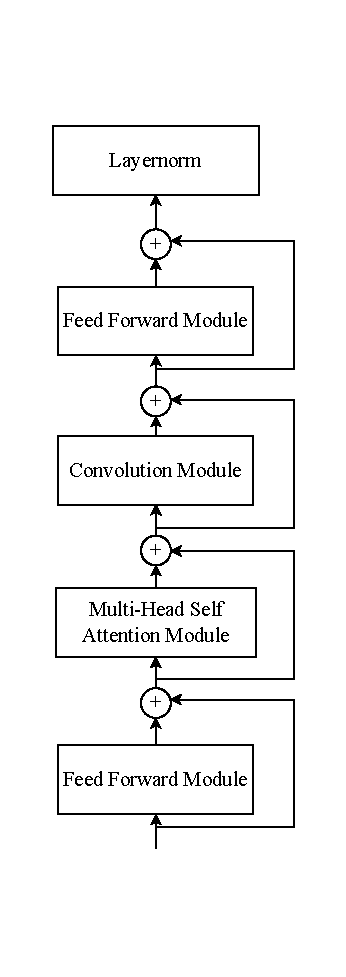
\includegraphics[scale=1]{Images/ASR/Methodology/ASR-ConformerBlock.drawio.pdf}
        \caption{Conformer Architecture}
    \end{figure}
The acoustic modelling element of the two ASR systems is the Conformer encoder. It works by stacking several of the same ConformerLayer blocks and each block is an assembly of multi-headed self-attention and local convolutional processing in a sandwich structure of macaron nets. FastConformer encoder employs 16 layers and the model dimension is 176 whereas IndicConformer encoder employs 17 layers and its model dimension is 512. Each layer has the same structure, and it is just the size that is different.

Every ConformerLayer has five sub-modules used in sequence, where first Feed Forward Module (FFN1), a Multi-Headed Self-Attention Module (MHSA), a Convolution Module (Conv), a second Feed Forward Module (FFN2), and a final Layer Normalisation. This structure, based on Macaron-Net, encircles the attention and convolution modules between two half-weighted feed-forward modules enabling the model to detect both regional and global speech patterns in a combined expression.

\textbf{Feed Forward Module}

The Conformer architecture requires the Feed Forward Module to deal with features at single-token level. It includes two FFNs that work in the same way, one before and one after the focus on attention and convolutional techniques. They function as processes before and after training to boost the model’s ability to learn features and still use few resources. All FFNs include certain layers in their structure: layer normalization, transformations, activation, and residual connections.

All FFNs start off with layer normalization , ensuring that the mean and variance of the input are stable. In doing this step, the inputs to the next layers become more controlled, making the whole training process more stable. Once the module is normalized, it goes on to use a linear transformation followed by a non-linear GeLU or ReLU function. This way, the model can represent situations that are not simple, but more complex. After the activation, the results are passed through a linear layer that reshapes them to the original number of features. To sum up, residual connections enable gradients to continue, making sure issues like vanishing gradients are not a problem during training.

\textbf{Multi-Headed Self Attention Module}

    \begin{figure}[H]
        \centering
        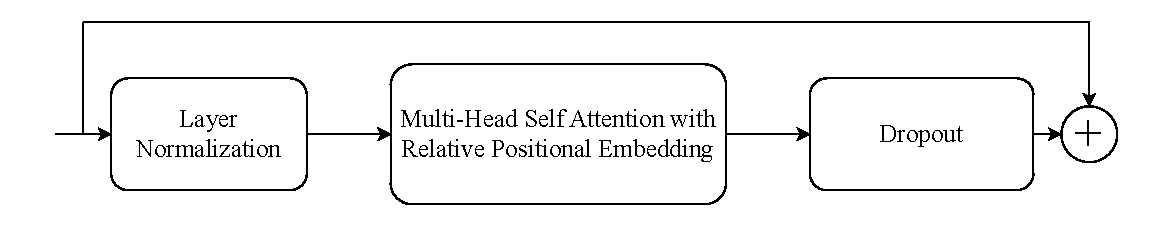
\includegraphics[width=\linewidth]{Images/ASR/Methodology/ASR-MultiHeadedSelfAttentionModule.drawio.pdf}
        \caption{Block Diagram of Multi-Headed Self Attention Module Architecture}
    \end{figure}

\textbf{Multi-Head Self Attention with Relative Positional Embedding}

    \begin{figure}[H]
        \centering
        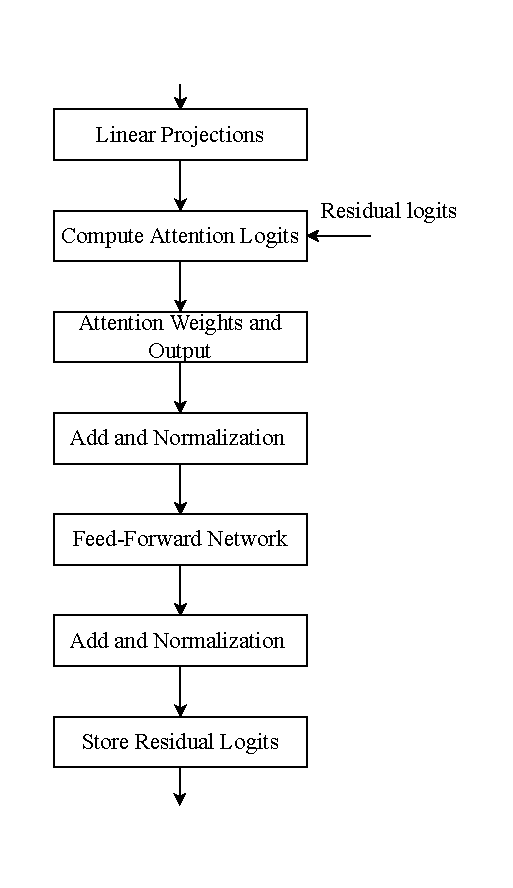
\includegraphics[scale=1]{Images/ASR/Methodology/ASR-ResMHA.drawio.pdf}
        \caption{Block Diagram of Multi-Head Self Attention with Relative Positional Embedding}
    \end{figure}
The self-attention sub-module gives attention to the long distance relationships in the entire sequence of the speech. It employs Relative Position Multi-Head Attention, which adds relative positional encoding to the attention score computation instead of appending some fixed absolute positional encoding to the input. This enables the model to extrapolate to utterances of varying lengths and also to be sensitive to the relative position of the frames instead of the absolute position of the frame within the sequence.
There are four known linear projections in the attention module which include query (Q), key (K), value (V) and output that all take place in the hidden dimension of the model. One more linear projection (linear\_pos) gives positional bias terms utilized in the calculation of the relative attention score. The attention weights are dropped (p=0.1). Layer Normalization comes before the module. The specific dimensions are:
\begin{itemize}
    \item \textbf{Fast Conformer(English)}:  All projections are Linear(176, 176). With a model dimension of 176 and 4 attention heads, each head operates over a 44-dimensional subspace.

    \item \textbf{Indic Conformer(Nepali)}: All projections are Linear(512, 512). With a model dimension of 512 and 8 attention heads, each head operates over a 64-dimensional subspace.
\end{itemize}
 
\textbf{Convolution Module}
    \begin{figure}[H]
        \centering
        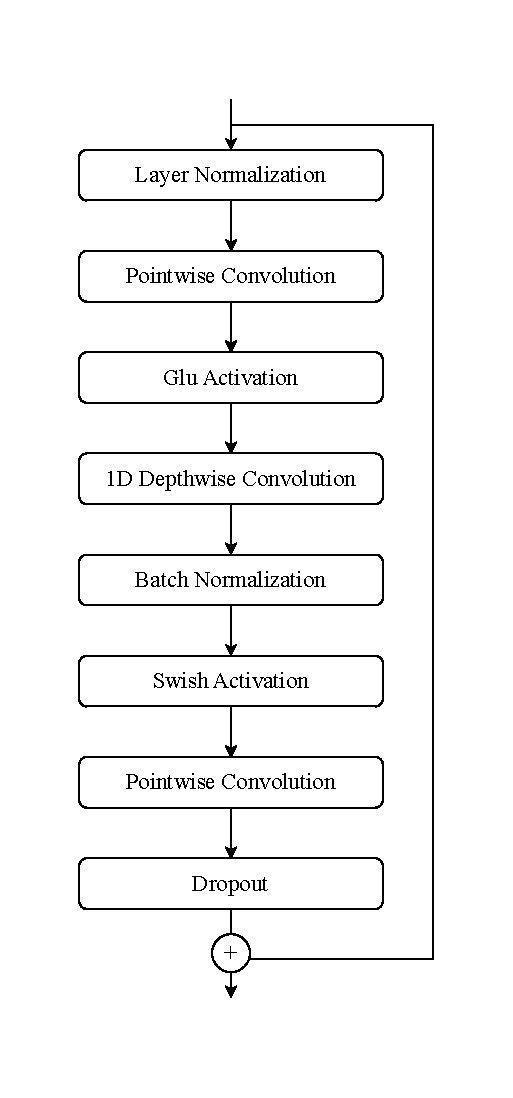
\includegraphics[scale=1]{Images/ASR/Methodology/ASR-Convolution Module.drawio.pdf}
        \caption{Block Diagram of Convolution Module}
    \end{figure}
    \begin{enumerate}
        \item \textbf{Pointwise Convolution}

        Part of the convolutional modules makes use of pointwise convolution to reorganize feature representations efficiently. A pointwise convolution also known as 1x1 convolution works by running a convolutional filter over all input channels with a kernel size of 1. In Conformer, time is what is being transformed in the temporal dimension of the speech features. One of the main uses of pointwise convolution is to keep the input’s spatial or temporal features while transforming it to a different dimension. 
        
        With pointwise convolutions, the Conformer saves computations and improves model performance, since it skips costly spatial computations.

        \item \textbf{GLU Activation}

        The GLU activation function is added to bring non-linearity and make the features better represented. The input is separated into two pieces, and the “gate” part gets processed by a sigmoid function, then those values are multiplied with the remaining data. Because of gating, the model can control information being exchanged and give more attention to significant elements as needed. By using GLU on the feed-forward and convolutional layers in the Conformer increases the ability to represent speech data while maintaining a good balance between simplicity and complexity.

        \begin{figure}[H]
            \centering
            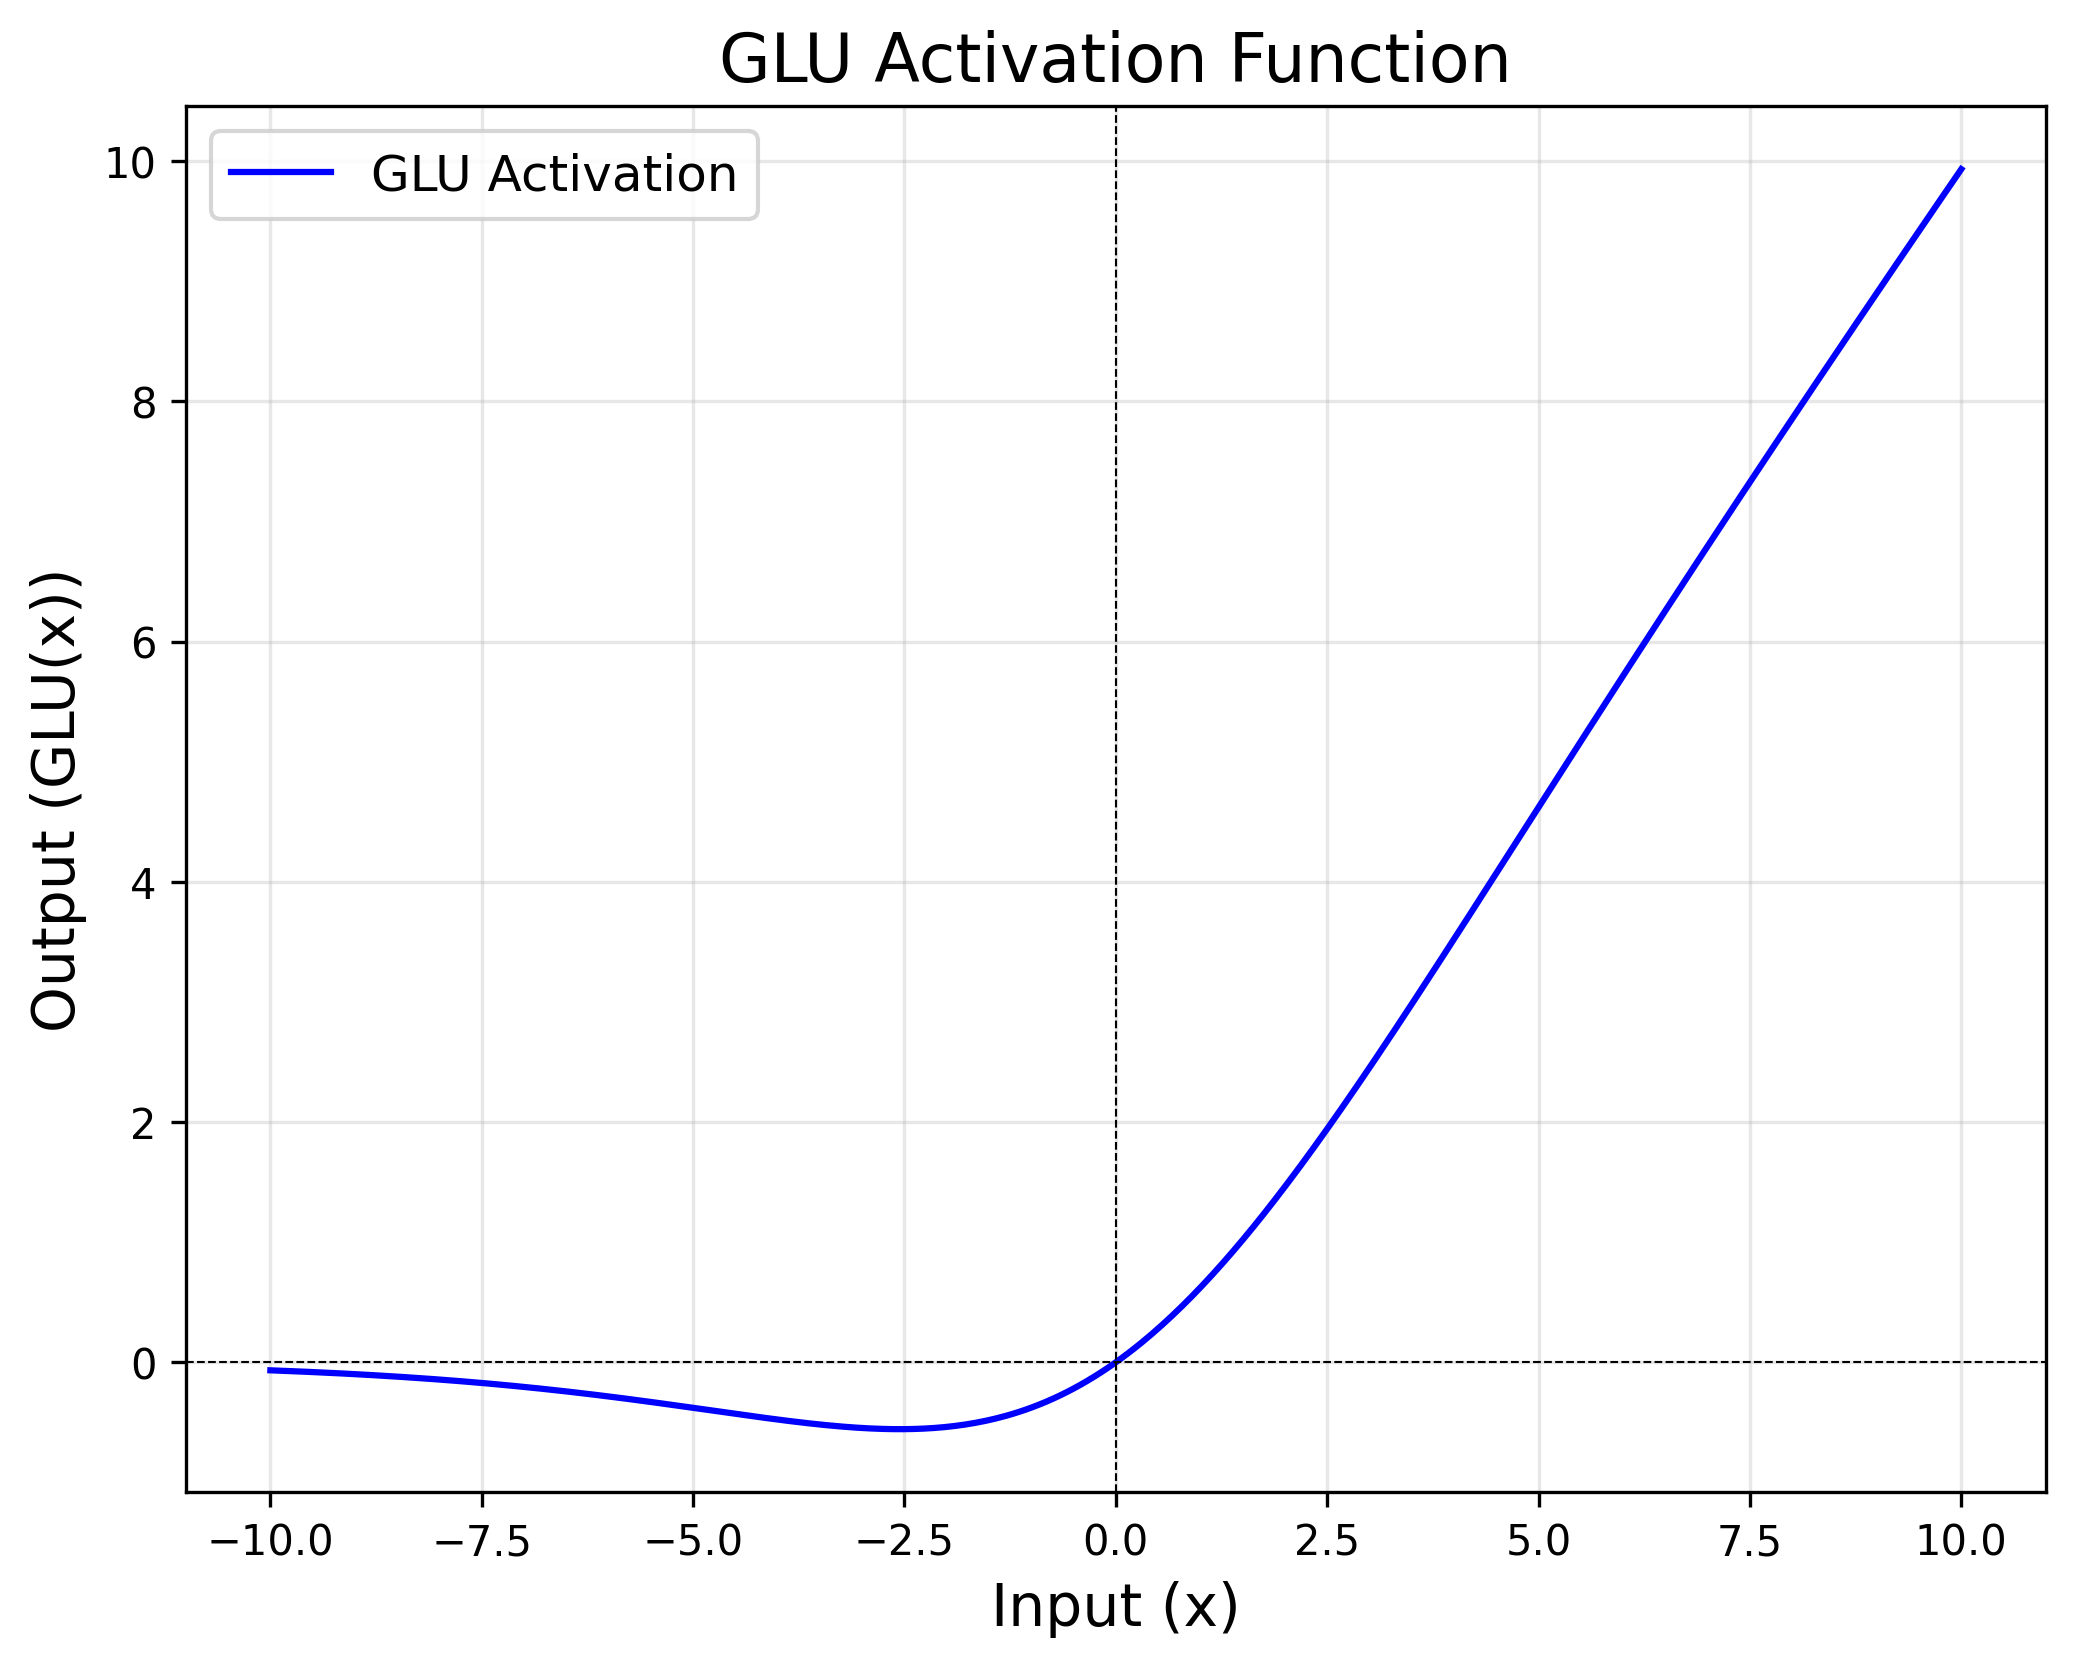
\includegraphics[width=\linewidth]{Images/ASR/Methodology/glu_activation.png}
            \caption{Graph of GLU activation}
        \end{figure}
        
        \begin{figure}[H]
            \centering
            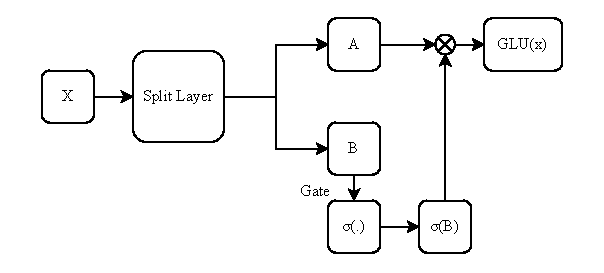
\includegraphics[width=\linewidth]{Images/ASR/Methodology/ASR-GLU.drawio.pdf}
            \caption{Block Diagram of GLU activation}
        \end{figure}
        
        
        \item \textbf{1D depthwise convolution}

        The Conformer designs 1D depthwise convolution to catch the connections between parts of speech by filtering each channel in sequence along the time axis. Consequently, resources are saved without losing the following local features. It combines pointwise convolution to help channels connect, thus it works well for modeling features in successive speech.

        \item \textbf{Swish Activation}

        The Swish activation function is well known in deep learning since it performs better than simpler activation functions like ReLU (Rectified Linear Unit). Swish is useful in the Conformer architecture because it boosts both the strength and speed of training for automatic speech recognition tasks.
        Swish is defined as:
        \begin{equation}
            \text{Swish}(x) = x \cdot \sigma(x)
        \end{equation}

        \begin{figure}[H]
            \centering
            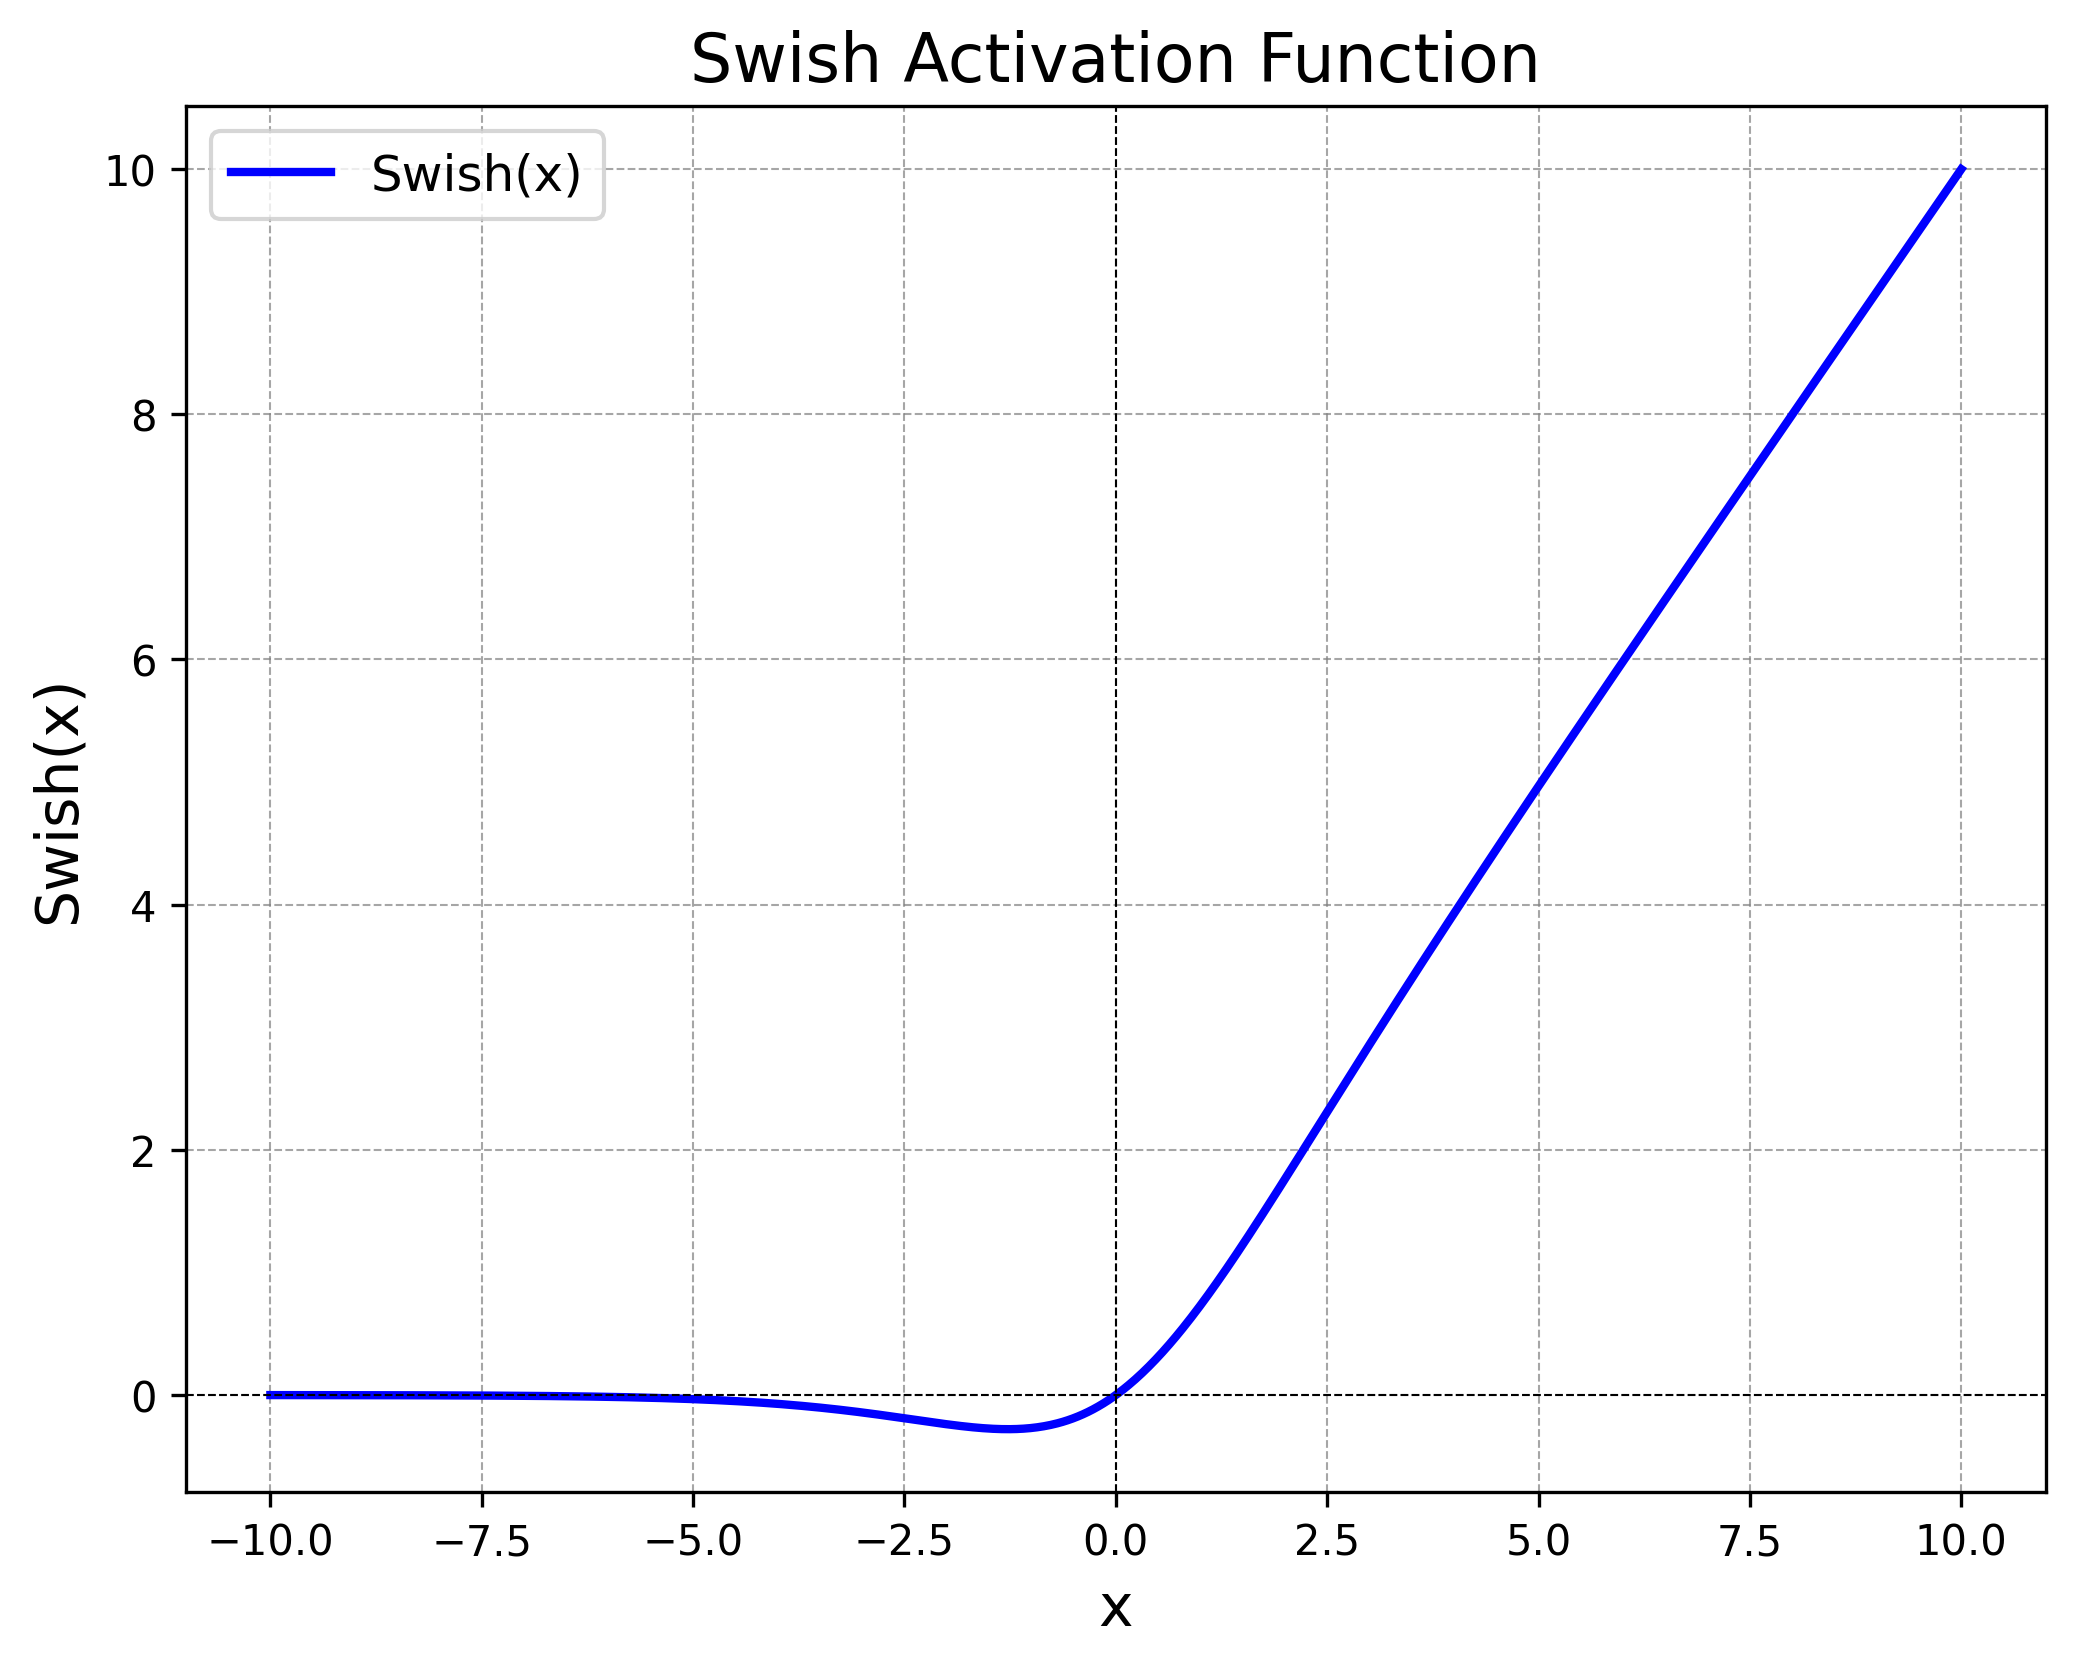
\includegraphics[width=\linewidth]{Images/ASR/Methodology/swish_activation.png}
            \caption{Graph of Swish Activation} \end{figure}
    \end{enumerate}
    
\textbf{Layer Normalization}\\
The purpose of Layer Normalization is to keep the training stable and speedy by normalizing the activations in all layers. To be clear, it standardizes each input value in every feature dimension (the hidden dimension) for each step. This lets the mean and variance of the activations not change, so problems with vanishing or exploding gradients are avoided. It is applied in many places in the network to make sure the gradients do not experience fluctuations. As internal covariate shift is limited, the model performs better at obtaining strong features from speech data, seen mainly in deep networks with lots of layers. This method becomes crucial for reaching consistent and efficient convergence in automatic speech recognition. 

\textbf{Conformer Block Computation}\\
Our proposal for Conformer includes putting the Multi-Headed Self-Attention and the Convolution modules between two Feed Forward modules. Macaron-Net \cite{macaron} was a motivation behind this sandwich structure, and it suggests removing the regular feed-forward layer from a normal Transformer block and placing two reduced-size feed-forward layers, one before and another after the attention layer. Like in Macron-Net, we add half-step residual weights to the feed-forward (FFN) parts of our model. The second feed-forward module comes ahead of the last layernorm layer. In math terms, yi is the output produced by Conformer block i as it takes input xi as input.
     
Mathematically, this means that for input $x_i$ to a Conformer block $i$, the output $y_i$ of the block is:
    \begin{align}
    \tilde{x}_i &= x_i + \frac{1}{2} \text{FFN}(x_i) \\
    x'_i &= \tilde{x}_i + \text{MHSA}(\tilde{x}_i) \\
    x''_i &= x'_i + \text{Conv}(x'_i) \\
    y_i &= \text{LayerNorm}\left(x''_i + \frac{1}{2} \text{FFN}(x''_i)\right)
    \end{align}

\subsubsection{SentencePiece Tokenizer}
Sentence Piece is a language-neutral subword tokenisation system that is actively used in end-to-end automatic speech recognition (ASR) systems to alleviate vocabulary sparsity and out-of-vocabulary (OOV) effects. SentencePiece is unlike tokenisers, which rely on whitespace, and works on an unsegmented stream of Unicode characters, where subword units are directly learned from the input. It is therefore especially beneficial when dealing with languages that do not have clear word delimiting boundaries and with infrequent or misspelt words in speech transcripts. The framework incorporates the use of either the Byte-Pair Encoding (BPE) as the base algorithms and thus enables one to trade-off the granularity of tokens and the general model performance. SentencePiece produces strong, compact representations, operating on a subset of corpora coded uniformly and reversibly into subword tokens, such as special symbols marking the start and end of an utterance, and these representations are compatible with the output of acoustic models in modern ASR pipelines.

\begin{algorithm}[H]
	\caption{Train SentencePiece Tokenizer (BPE)}
	
	\textbf{Input:} Raw training text, target vocabulary size, model type (BPE), special tokens \\
	\textbf{Output:} Trained tokenizer model, subword vocabulary, encoding and decoding rules
	
	1. Preprocess the training text by normalizing whitespace and optionally adding sentence boundary markers\;
	
	2. Initialize a character-level vocabulary using all unique Unicode symbols present in the text\;
	
	3. Add predefined special tokens (e.g., \texttt{<s>}, \texttt{</s>}, \texttt{<unk>}) to the vocabulary\;
	
	4. If the model type is BPE:
	\begin{itemize}
		\item Initialize all characters as individual tokens
		\item Convert the full text into a sequence of tokens based on the current vocabulary
		\item Repeat until the target vocabulary size is reached:
		\begin{itemize}
			\item Count the frequency of all adjacent token pairs
			\item Select the most frequent token pair
			\item Merge the selected pair into a new subword token
			\item Add the new token to the vocabulary
			\item Replace all occurrences of the merged pair in the token sequence
		\end{itemize}
	\end{itemize}
	
	5. Save the learned vocabulary, subword merge rules, and model parameters\;
	
	6. Return the trained tokenizer capable of encoding and decoding arbitrary text sequences\;
	
\end{algorithm}

\subsubsection{Connectionist Temporal Classification (CTC) Head}

Connectionist Temporal Classification (CTC) is commonly used in sequence-to-sequence
tasks such as speech recognition and handwriting recognition, where the input and
output sequences are of different lengths and are not pre-aligned. CTC can be used
both as a loss function during training and as a decoding strategy during inference.

CTC introduces a special \emph{blank symbol}, typically denoted as \( b \), which
allows the model to emit either an output symbol \( y_t \) or a blank at each time
step of the input sequence.

Let the input sequence be
\begin{equation}
	\mathbf{x} = (x_1, x_2, x_3, \dots, x_T),
\end{equation}
where \( T \) denotes the input sequence length, and let
\begin{equation}
	\mathbf{y} = (y_1, y_2, \dots, y_U)
\end{equation}
be the target output sequence.

CTC defines a collapsing function \( \mathcal{B} \) that removes repeated symbols
and blank symbols. The set of all alignment paths that collapse to \( \mathbf{y} \)
is denoted by
\begin{equation}
	\mathcal{B}^{-1}(\mathbf{y}).
\end{equation}
\begin{itemize}
    \item \textbf{Fast Conformer(English)}: Conv1d(176, 1025, kernel size=1). Projects the 176-dimensional encoder output to a 1025-token vocabulary (1024 BPE subword units + 1 blank token).

    \item \textbf{Indic Conformer(Nepali)}: Conv1d(512, 5633, kernel size=1). Projects the 512-dimensional encoder output to a 5633-token vocabulary (5632 BPE subword units + 1 blank token, with padding\_idx=5632).
\end{itemize}

\textbf{CTC Objective}

The conditional probability of the output sequence \( \mathbf{y} \) given the input
sequence \( \mathbf{x} \) is defined as
\begin{equation}
	P(\mathbf{y} \mid \mathbf{x}) =
	\sum_{\boldsymbol{\pi} \in \mathcal{B}^{-1}(\mathbf{y})}
	P(\boldsymbol{\pi} \mid \mathbf{x}),
\end{equation}
where \( \boldsymbol{\pi} = (\pi_1, \pi_2, \dots, \pi_T) \) represents an alignment path.

Each alignment probability is factorized over time steps as
\begin{equation}
	P(\boldsymbol{\pi} \mid \mathbf{x}) =
	\prod_{t=1}^{T} P(\pi_t \mid \mathbf{x}),
\end{equation}
with
\begin{equation}
	\pi_t \in \mathcal{Y} \cup \{ b \},
\end{equation}
where \( \mathcal{Y} \) is the output vocabulary and \( b \) denotes the blank symbol.

The summation over all valid alignments is efficiently computed using dynamic
programming techniques such as the forward--backward algorithm.

\textbf{Inference}

During inference, the output sequence is simplified by collapsing consecutive
repeated symbols and removing blank symbols. For example,
\begin{equation}
	\texttt{h\_l\_l\_o} \;\longrightarrow\; \texttt{hello}.
\end{equation}

\textbf{Comparison with Attention-Based Methods}

Unlike attention-based models that perform global alignment between input and output
sequences, CTC performs alignment locally at each time step. This local alignment
strategy avoids scanning the entire sequence during decoding, leading to improved
computational efficiency, especially for long input sequences.

\subsubsection{AdamW Optimizer}
AdamW is an improvement over the traditional Adam optimizer, as it decouples the
weight decay term from the gradient-based parameter updates, thereby enabling more
effective regularization. This property is particularly beneficial when training
large-scale deep learning models such as FastConformer, a highly efficient variant
of the Conformer architecture used in speech recognition.

In the standard Adam formulation, weight decay is applied through L2 regularization
of the loss, which can interfere with the adaptive learning-rate mechanism. AdamW
addresses this limitation by applying weight decay directly to the model parameters
after the Adam update step, as shown in the following equation:

\begin{equation}
	\theta_{t+1} = \theta_t
	- \eta \left( \frac{\hat{m}_t}{\sqrt{\hat{v}_t} + \epsilon} \right)
	- \eta \lambda \theta_t
\end{equation}

where \( \theta_t \) represents the model parameters at training step \( t \),
\( \eta \) is the learning rate, \( \hat{m}_t \) and \( \hat{v}_t \) are the
bias-corrected first and second moment estimates, respectively, and \( \lambda \)
denotes the weight decay coefficient.

In architectures such as FastConformer, which combine convolutional and
self-attention layers, training stability and generalization are critical. By
providing cleaner and more consistent regularization, AdamW typically leads to
better convergence behavior and improved generalization compared to the standard
Adam optimizer, especially when training transformer-based models with large batch
sizes and long input sequences.

\subsubsection{Cosine Annealing}
Cosine annealing is a non-linear learning rate-scheduling method, common in fine-tuning deep neural networks, and widely used to fine-tune pre-trained models of speech recognition, such as FastConformer. As compared to aggressive decay schemes, cosine annealing progressively decreases the learning rate according to a cosine curve, beneficial to maintaining knowledge acquired in the pre-trained weights but enabling a controlled adaptation to the target domain.
In the case of fine-tuning, the model parameters are already in a well-trained state (e.g. using large-scale training data, such as LibriSpeech). Any initial learning rate can be catastrophically forgetful or unstable, and a fixed low initial learning rate can result in underfitting. Cosine annealing is one way to solve this problem, with an initial small learning rate gradually reduced towards zero during the fine-tuning.

\begin{equation}
\eta_t
=
\eta_{\min}
+
\frac{1}{2}
\left(\eta_{\max} - \eta_{\min}\right)
\left(
1 + \cos\left(\frac{\pi t}{T}\right)
\right)
\end{equation}

\begin{itemize}
  \item $\eta_t$: learning rate at step or epoch $t$
  \item $\eta_{\max}$: initial (maximum) learning rate
  \item $\eta_{\min}$: minimum learning rate
  \item $t$: current step or epoch, $0 \leq t \leq T$
  \item $T$: total number of steps or epochs
\end{itemize}

\subsubsection{Greedy Decoding}
Greedy batch decoding which is an efficient inference strategy is used to perform transcription which is typically used in Connectionist Temporal Classification (CTC) based Automatic Speech Recognition (ASR) systems. Greedy decoding chooses the most likely token at a time step without one looking at other hypotheses or context. This process can be optimized by the so-called batch (greedy\_batch) variant, which applies parallelized decoding of many audio samples but in that instance to one file with batch\_size=1 to be compatible and to have slight efficiency improvements.
Greedy decoding, in contrast to more advanced approaches like beam search, does not have a pool of candidate sequences, and thus is unable to combine external knowledge such as language models. It consequently can achieve low latency and high performance, but can result in lower fluent or grammatically irregular outputs, notably under noisy environments, or on ambivalent acoustic inputs. The method is based on the fact that the model (here a FastConformer) is only able to directly decode audio features into subword units (BPE tokens) and then decodes without rescoring or language improvement.
Therefore, it is a system that gives more focus to computational performance and simplicity than to the linguistic quality, so that it can be used in real-time-sensitive applications or in other situations where speed is paramount and minor mistakes in the transcription are tolerable.

\subsubsection{Softmax Function}
Softmax function helps convert raw logits from the output layer into a distribution of probabilities for the target vocabulary. This means the model creates probabilities for every output token (such as phonemes, characters or words) and, during decoding, it can pick the most likely sequence.

\begin{equation}
\text{softmax}(z_i) = \frac{e^{z_i}}{\sum_{j=1}^{K} e^{z_j}}
\end{equation}

\begin{itemize}
  \item \( z_i \): The input score (logit) for class \( i \)
  \item \( z_j \): The input score (logit) for class \( j \)
  \item \( K \): The total number of classes
\end{itemize}

\subsubsection{Word Error Rate (WER)}
Word Error Rate (WER) is the most popular metric used to evaluate the performance of the Automatic Speech Recognition (ASR) systems. It is used to measure the accuracy of transcription by comparing the hypothesis of the system to a ground-truth reference transcript.


\begin{equation}
	\text{WER} = \frac{S+D+I}{N}
\end{equation}

where,
\begin{itemize}
	\item S = Number of substitutions (wrong words)
	\item D = Number of deletions (missing words)
	\item I = Number of insertions (extra words)
	\item N = Total number of words in the reference
\end{itemize}
